\documentclass{beamer}
% \RequirePackage[T2A]{fontenc}
\RequirePackage[utf8]{inputenc}
\RequirePackage[english,russian]{babel}

\usepackage{listings}
\usepackage{courier}
\usepackage{tikz}
\usepackage{float}
\usepackage{graphicx}
\usepackage{epstopdf}

\usepackage{algorithm2e}

 % Перевод плагина
\SetKwInput{KwData}{Input parameters}
\SetKwInput{KwResult}{Result}
\SetKwInput{KwIn}{Input data}
\SetKwInput{KwOut}{Output Data}
\SetKwIF{If}{ElseIf}{Else}{if}{then}{else\ if}{else}{end\ of\ condition}
\SetKwFor{While}{while}{execute}{end\ of\ loop}
\SetKw{KwTo}{to}
\SetKw{KwRet}{return}
\SetKw{Return}{return}
\SetKwBlock{Begin}{begin\ block}{end\ block}
\SetKwSwitch{Switch}{Case}{Other}{Check\ a\ value}{and\ execute}{a\ case}{otherwise}{end\ of\ case}{end\ of\ value\ check}
\SetKwFor{For}{loop}{execute}{end\ of\ loop}
\SetKwFor{ForEach}{for\ each}{execute}{end\ of\ loop}
\SetKwRepeat{Repeat}{repeat}{while}
\SetAlgorithmName{Algorithm}{algorithm}{List of algorithms}


\usetikzlibrary{shapes,arrows}

%\usetheme{CambridgeUS}%{Warsaw}
%\usetheme {Madrid}
%\useoutertheme {shadow}
%\usecolortheme{beaver}%{structure черный}%{seagull серый}%{lily желтый}%{beaver красный}
%\usefonttheme{structurebold}
%\setbeamerfont{framesubtitle}{size=\large}
%\useoutertheme{infolines}
%\useoutertheme{split}
%I DONT WANT TO SEE THOSE NAVIGATION SYMBOLS
%\setbeamertemplate{navigation symbols}{}

\mode<presentation>
{
    \usefonttheme[onlymath]{serif}
\usetheme {Madrid}
%\useoutertheme {shadow}
%\usecolortheme{beaver}%{structure черный}%{seagull серый}%{lily желтый}%{beaver красный}
\usefonttheme{structurebold}
\setbeamerfont{framesubtitle}{size=\large}
\useoutertheme{infolines}
%\useoutertheme{split}
%I DONT WANT TO SEE THOSE NAVIGATION SYMBOLS
\setbeamertemplate{navigation symbols}{}
\setbeamertemplate{footline}
}

\setbeamercolor{color1}{bg=red!40!green,fg=black}
\setbeamercolor{uppercol}{fg=white,bg=brown}

\title{Control Flow Graph Visualization in\\ Compiled Software Engineering}

\author[A.~Mikhailov]{Andrey Mikhailov${}^{*}$, Aleksey Hmelnov${}^{*}$, Evgeny Cherkashin${}^{*\;**}$ and Igor Bychkov\\\texttt{\scriptsize{\{mikhailov,alex,eugeneai,bychkov\}@icc.ru}}}

\institute[ИДСТУ СО РАН]
{
    Институт динамики систем и теории управления Сибирского отделения Российской академии наук (ИДСТУ СО РАН)\\
    \vspace{0.7cm}
}

\date{\scriptsize{
\\
    \vspace{0.3cm}}
ISDCT SB RAS, INRTU
\\
31 May 2016
\\
Opatija, Croatia
}
\begin{document}

%\титульный
\section{Delphi}
\maketitle

%\граф потоков управления

\section{Delphi}
\begin{frame}
\frametitle{Control flow graph}

\tiny{

\newtheorem{Def}{Определение}[section]
\begin{Def}
Ориентированный граф $G(X,U)$ называется графом потоков управления, если выполняются следующие условия:

	\begin{enumerate}
		\item[1)]
		граф $G$ не содержит параллельных дуг;
		\item[2)]
		в множестве вершин графа выделена одна вершина $start$, которая является входом графа;
		\item[3)]
		в множестве вершин графа выделена одна вершина $end$, которая является выходом графа;
		\item[4)]
		каждая вершина $x \in X$ достижима из $start$;
		\item[5)]
		из каждой вершины $x \in X$ достижима вершина $end$;
	\end{enumerate}
\end{Def}

\newtheorem{DOM}{Определение}[section]
\begin{Def}
	Узел $x$ является доминатором $y$ ($x$ $dom$ $y$) в направленном графе, если любой путь от $start$ до $y$ включает узел $x$.
\end{Def}

\newtheorem{IDOM}{Определение}[section]
\begin{Def}
	Узел $x$ является непосредственным доминатором $y$ ($x$ $idom$ $y$), если $x$ $dom$ $y$, и не существует такого промежуточного узла $P$, что $x$ $dom$ $P$ и $P$ $dom$ $y$.
\end{Def}

}
\end{frame}

%\ иерархический раскладчик

\section{Delphi}
\begin{frame}
\frametitle{Метод поуровнего изображения направленных графов (иерархический раскладчик)}
\scriptsize{

uDraw (daVinci), VCG, Graphlet, GraVis, Graph Drawing Server, graphViz, VisualGraph

\begin{enumerate}
	\item \textbf{Распределение вершин по уровням.} Каждой вершине присваивается ее ранг. При этом все дуги могут следовать только от меньшего ранга к большему. Между вершинами одного ранга не может быть дуг. Для распределения рангов вершин могут использоваться различные методы, в простейшем случае в качестве ранга может быть использована длина пути при обходе в глубину.
	\item \textbf{Определение порядка вершин на уровнях.} Вершины упорядочиваются внутри уровня таких образом, чтобы минимизировать количества пересечений дуг. Самым распространенным способом решения этой задачи является <<метод медиан>>.
	\item \textbf{Определение координат вершин на уровне.} На каждой уровне каждой вершине присваиваются координаты таким образом, чтобы граф соответствовал определённым для него эстетическим критериям.
	\item \textbf{Проведение дуг.}	Обычно, эту задачу выделяют в отдельный этап, только в том случае, если дуги изображаются не в виде прямых.
\end{enumerate}
}
\end{frame}

%\критерии качества визуализации

\section{Delphi}
\begin{frame}
\frametitle{Критерии качества визуализации гарфа}
\tiny{
	\newtheorem{vis}{Определение}
	\begin{vis}
	Раскладка графа на плоскости (или в пространстве) — это отображение вершин и ребер графа в множество точек плоскости (или пространства).
	\end{vis}

	\begin{itemize}
	\item \textit{Изобразительное соглашение} — это одно из основных правил, которому должно удовлетворять изображение графа, чтобы быть допустимым.

	\item \textit{Эстетические критерии} определяют такие свойства изображений, которые желательно применять в наибольшей степени, насколько это возможно, чтобы повысить наглядность изображения.

	\item \textit{Ограничения.} Если соглашения и эстетические критерии формулируются по отношению ко всему графу и его изображению, то ограничения относятся к отдельным подграфам и частям изображений.
\end{itemize}

	\begin{figure}[htbp]
		\centering
			
\includegraphics[width=0.50\textwidth]{Pic/Pic1.eps}
		\caption{Разные способы визуализации одного и того же графа}
		\label{fig:VisExample}
	\end{figure}
}
\end{frame}

%\изобразительные соглашения

\section{Delphi}
\begin{frame}
\frametitle{Изобразительные соглашения для уграфа}
\footnotesize{
	\begin{enumerate}
		\item[а)]
			\textbf{Блок действия.}  Представляет собой узел, передача управления из которого осуществляется только в одном направлении.
		\item[б)]
			\textbf{Логический блок (блок условия).} Соответствует условному оператору в высокоуровневых языках, а в графе узлу расхождения потока управления.
		\item[в)]
			\textbf{Граница цикла.} Состоит из двух частей, обозначающих начало и конец операций, выполняемых внутри цикла.
		\item[г)]
			\textbf{Блок начало-конец (пуск-остановка).} Отображает вход и выход в функцию (программу).
	\end{enumerate}
}
\begin{figure}[htbp]
	\begin{minipage}[b]{0.24\linewidth}
	\center{
\includegraphics[width=0.35\textwidth]{Pic/BlocksA.eps} \\ а) блок действия}
	\end{minipage}
\hfill
\begin{minipage}[b]{0.24\linewidth}
	\center{
\includegraphics[width=0.35\textwidth]{Pic/BlocksB.eps} \\ б) логический блок}
	\end{minipage}
\begin{minipage}[b]{0.24\linewidth}
	\center{
\includegraphics[width=0.5\textwidth]{Pic/BlocksC.eps} \\ в) границы цикла}
	\end{minipage}
\begin{minipage}[b]{0.24\linewidth}
	\center{
\includegraphics[width=0.35\textwidth]{Pic/BlocksD.eps} \\ г) начало-конец}
	\end{minipage}
	\caption{Типы элементов.}
	\label{fig:Blocks}
\end{figure}
\end{frame}

%\TT регион

\section{Delphi}
\begin{frame}
\frametitle{TT - регион}

\scriptsize{
\newtheorem{TT}{Определение}[section]
\begin{Def}
	TT-регион (Two Terminal Region) --- это подграф в управляющем графе, который имеет один вход и один выход.
\end{Def}

\newtheorem{TTreg}{Определение}[section]
\begin{Def}
	Пара узлов $(a, b)$ управляющего графа $G$ образует TT-регион (Two Terminal), если
	\begin{enumerate}
		\item[1)]
			$a$ idom $b$;
		\item[2)]
			$b$ postidom $a$;
		\item[3)]
			любой цикл в управляющем графе, содержащий $a$, содержит также и $b$, и наоборот;
	\end{enumerate}
\end{Def}


\begin{figure}[htbp]
	\centering
		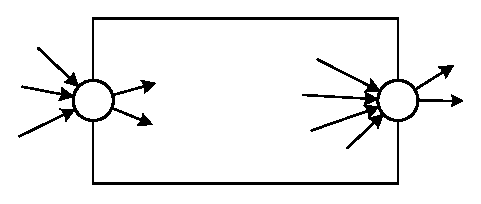
\includegraphics[width=0.5\textwidth]{Pic/TTRegion.eps}
	\caption{TT-регион}
	\label{fig:TTRegion}
\end{figure}
}

\end{frame}

%\выделяемые регионы

\section{Delphi}
\begin{frame}
\frametitle{Выделяемые регионы}
\begin{figure}[htbp]
	\centering
		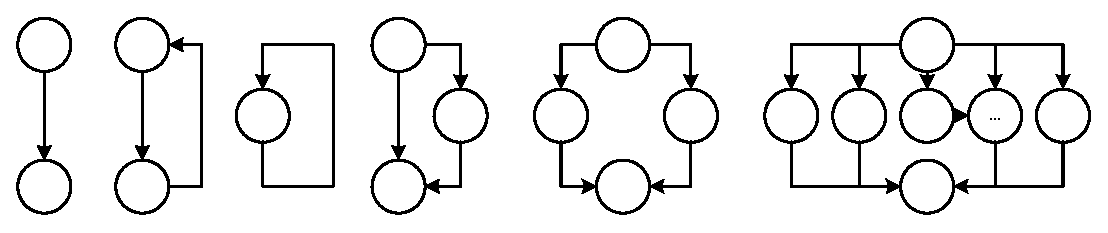
\includegraphics[width=1\textwidth]{Pic/Reg.eps}
	\caption{Выделяемые шаблоны}
	\label{fig:Regions}
\end{figure}
\end{frame}

%\алгоритм структурирования

\section{Delphi}
\begin{frame}
\frametitle{Изобразительные соглашения}
\small{%
\begin{algorithm}[H]
\SetAlgoLined %% Connects logical parts with lines
\KwData{G, D, P}
\KwResult{An abstract node containing a hierarchy of folded subgraphs}
%\While{$|E| \neq 0$ и $|V| \neq 1$}{
	\ForEach{$v \in D$ in a backward breadth-first order}{
		\ForEach{$p \in Children(v)$}{
			\If{$p\quad pidom\quad v$}{
				$S \leftarrow Children(v) \setminus p $ \\
				\If{$Classify\_Region(S) \neq \textit{undeterminated}$}{
					$Apply\_Template(S)$
				}\Else{
					$Hierarchical\_Layout(S \cup p)$ \\
					$Recognize\_Undeterminanted\_Region(S)$
				}
				$Modify(G,D,P)$
			}
		}
	}
%}
\caption{Algorithm of control flow graph structuring}
\label{alg:struct}
\end{algorithm}%
}
\end{frame}

%\Визуализация

\section{Delphi}
\begin{frame}
\frametitle{Процесс раскладки}

\small{Процесс раскладки происходит рекурсивно сверху вниз, начиная с региона верхнего уровня. Для этого региона задаются начальные координаты. Далее, если у региона есть шаблон, применяются правила отображения, определенные в нем.}

\begin{figure}[htbp]
	\centering
		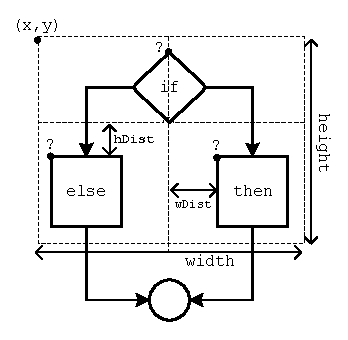
\includegraphics[width=0.4\textwidth]{Pic/IfThenElse.eps}
	\caption{Шаблон отображения if-then-else}
	\label{fig:IfThenElse}
\end{figure}

\end{frame}

%\Результат раскладки

\section{Delphi}
\begin{frame}
\frametitle{Результат раскладки}
\begin{figure}[htbp]
	\begin{minipage}[b]{0.49\linewidth}
	\center{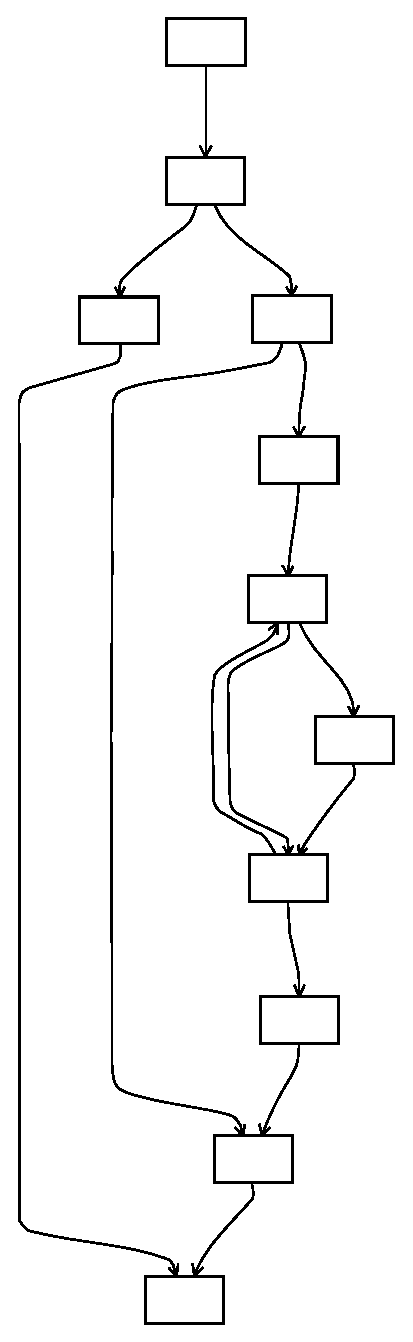
\includegraphics[width=0.35\textwidth]{Pic/Hier.eps} \\ а) Иерархический раскладчик}
	\end{minipage}
\hfill
\begin{minipage}[b]{0.49\linewidth}
	\center{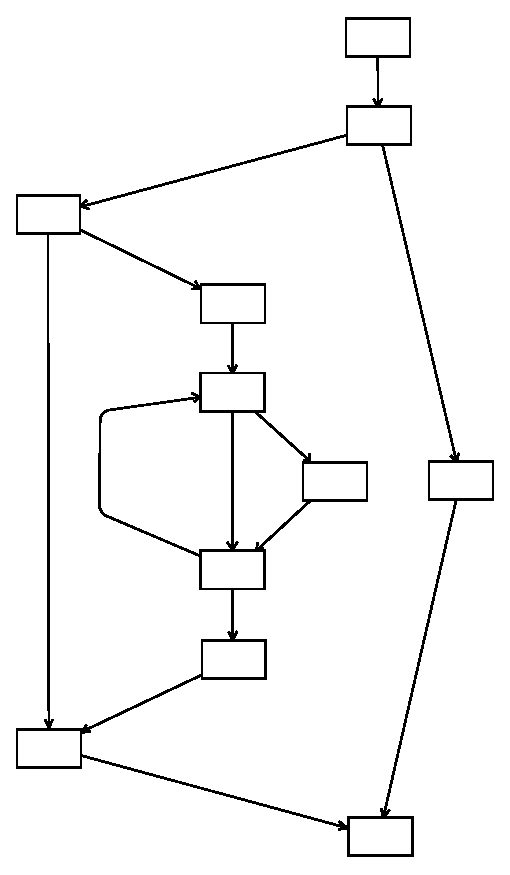
\includegraphics[width=0.5\textwidth]{Pic/Struct.eps} \\ б) Структурный раскладчик}
	\end{minipage}
	\tiny{
	\caption{Результат раскладки управляющего графа.}
	}
	\label{fig:image1}
\end{figure}
\end{frame}

%\Тестирование

\section{Delphi}
\begin{frame}
\frametitle{Результаты тестирования}
\footnotesize{
\begin{itemize}
	\item 197.parser\footnote{Синтаксический разбор для естественного языка}
	\item 252.eon\footnote{Трассировка лучей}
\end{itemize}

В результате около 70\% графов удалось структурировать полностью (не содержат <<неопределенных>> регионов). Около 96\% всех выделенных регионов являются структурными.

Основными преимуществами данного раскладчика являются:
\begin{itemize}
	\item Простота изменения правил визуализации графа посредством задания правил отображения шаблонов.
	\item Однообразное отображение подграфов, соответствующих одним и тем же операторам в высокоуровневых языках программирования.
	\item Возможность выделять специальным образом узлы и дуги графа, используя семантику, полученную в процессе структурирования графа.
\end{itemize}
}
\end{frame}


\section{Delphi}
\maketitle

\end{document}

%%% Local Variables:
%%% mode: latex
%%% TeX-master: t
%%% End:
